\newcommand{\handwrittenNoteBelow}[3]{
	\node[goetheblau, anchor=west, align=left] at ($(#1)+(1.6,-0.6)#3$) {\Large \Fontauri\bfseries #2};
	\path[<-, draw, goetheblau, ultra thick, bend right=15] ($(#1)#3$) to ++(1.5,-0.5);
}

\newcommand{\handwrittenNoteAbove}[3]{
	\node[goetheblau, anchor=west, align=left] at ($(#1)+(1.6,0.6)#3$) {\Large \Fontauri\bfseries #2};
	\path[<-, draw, goetheblau, ultra thick, bend left=15] ($(#1)#3$) to ++(1.5,0.5);
}


\begin{frame}{}
	\begin{center}
		\Huge
		\only<1>{Turing Maschine}
		\only<2-3>{%
			\only<2>{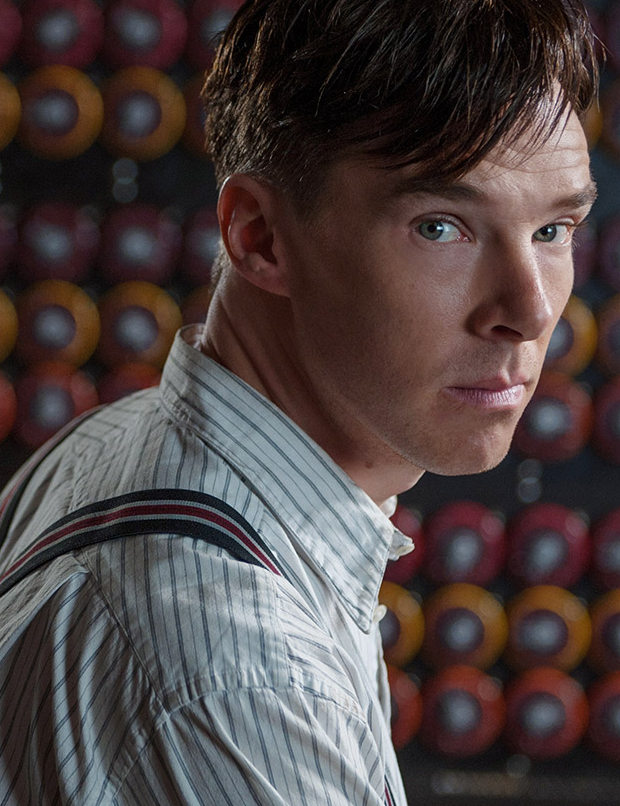
\includegraphics[height=0.6\textheight]{images/cumberbatch.jpg}}%
			\only<3>{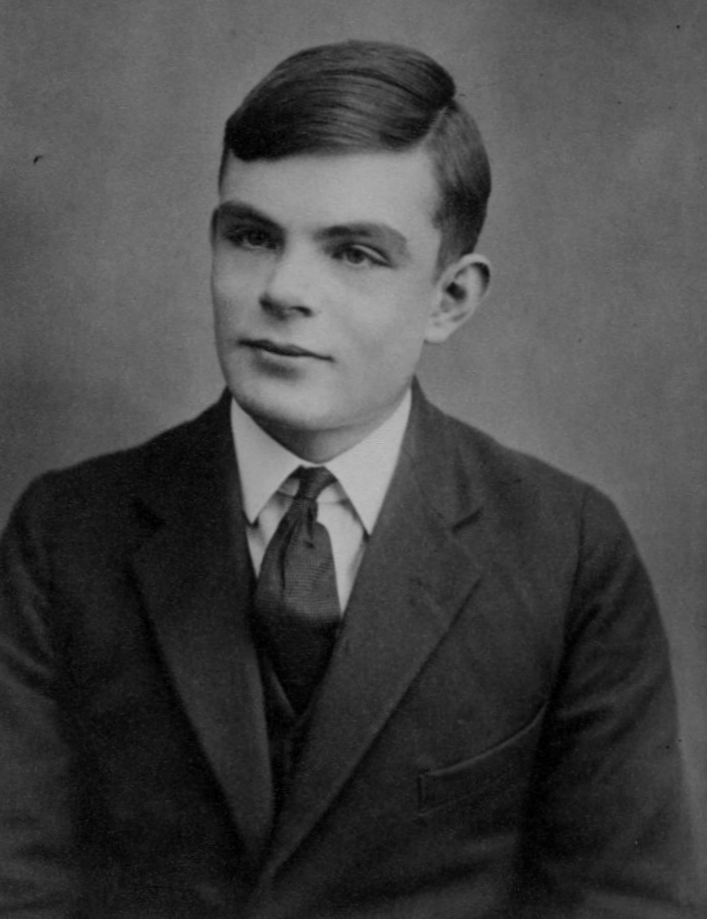
\includegraphics[height=0.6\textheight]{images/turing.jpg}}%
			\hspace{2em}
			
\includegraphics[height=0.6\textheight]{images/nos2012.jpg}
			\vspace{1em}
						
			Alan M. Turing\\
			1912 -- 1954 
		}
		\only<4>{
			\fbox{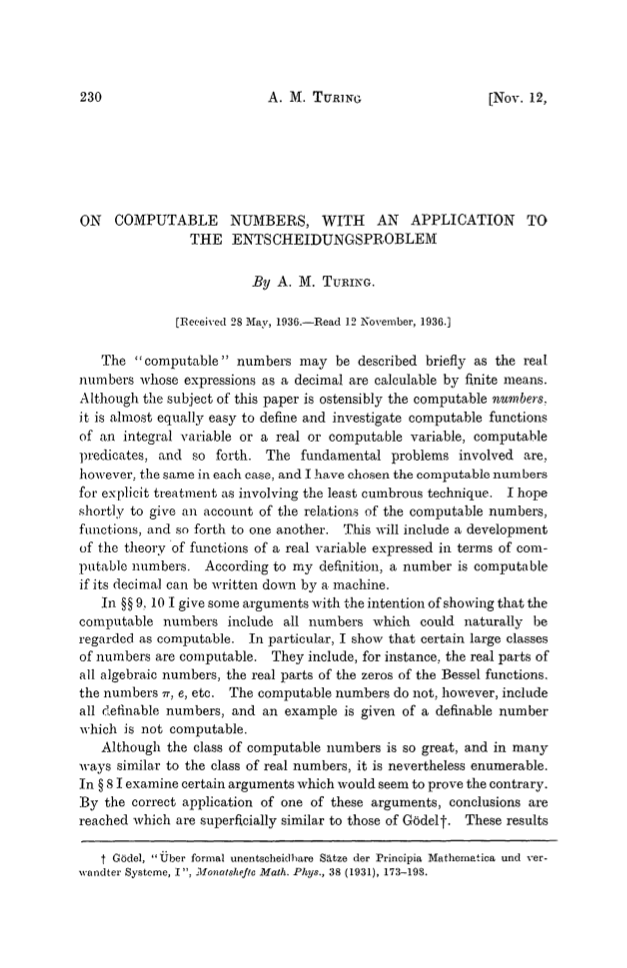
\includegraphics[height=0.6\textheight]{images/turing1936.png}}
			\vspace{1em}
			
			\textquotedblleft On Computable Numbers, With an Application to the Entscheidungsproblem\textquotedblright\\
			\textcolor{goetheblau}{[A. Turing, 1936/37]}
		}
	\end{center}
\end{frame}


\begin{frame}{Turing Maschine}
	\begin{center}
		\vspace{2em}

		\uncover<7->{
			\begin{tikzpicture}[remember picture]
				\node[tmState, draw] (stateA) {Zustand A};
				\node[tmState, draw, anchor=west] (stateB) at ($(stateA.east) + (5,0)$)  {Zustand B};
				
				\path[draw, ->, thick, bend left=10, shorten >=5pt, onslide={<8>, emorot}] (stateA) to node[above] {\tikzanchor{transAnchor} \texttt 0 zu \texttt 1, $\Rightarrow$} (stateB);
				\path[draw, ->, thick, bend left=10, shorten >=5pt] (stateB) to node[below,align=left] {\texttt 0 zu \texttt 0, $\Leftarrow$ \\ \texttt 1 zu \texttt 1, $\Leftarrow$} (stateA);
			\end{tikzpicture}

			\begin{tikzpicture}[remember picture, overlay]
				\handwrittenNoteBelow{stateB}{Programm}{-(2,1)}
							
			
				\only<8->{
					\handwrittenNoteAbove{transAnchor}
					{\normalfont\normalsize Wenn \textcolor{emorot}{\texttt 0} gelesen:\\ Schreibe \textcolor{emorot}{\texttt 1}, Kopf nach rechts}
					{+(1.8,0.2)}
				}
			\end{tikzpicture}			
		}

		\vspace{3em}
		
		\begin{tikzpicture}[
			remember picture
		]
			\node[tmCell                ] (tmbandcell0) {};		

			\foreach \x  [count=\i] in {
				0,0,1,
				\only<2->{--},
				\only<2->{\#},
				\only<2->{c},
				\only<2->{o},
				\only<2->{v},
				\only<2->{f},
				\only<2->{e},
				\only<2->{f},
				\only<2->{e}
			} {
				\node[tmCell] at ($(tmbandcell0) + (\i*\cellSize,0) - (\cellSize,0)$) {\x};
			}
		\end{tikzpicture}
			

		\begin{tikzpicture}[overlay, remember picture]
			\only<1-2> {
				\handwrittenNoteBelow{tmbandcell0}{Eingabe}{+(2, -0.6)}
			}
		
			\only<1> {\tmDrawGrid{0}{3}}
			\only<2> {\tmDrawGrid{0}{12}}
			\only<3-> {
				\foreach \i in {1,...,5} {
					\node[tmCell, tmCellBlank] at ($(tmbandcell0) - (\i*\cellSize,0)$) {\only<4->{\tmBlankSym}};
					\node[tmCell, tmCellBlank] at ($(tmbandcell0) + (\i*\cellSize,0) + (11*\cellSize, 0)$) {\only<4->{\tmBlankSym}};
				}
				\tmDrawGrid{-5}{18}

				\handwrittenNoteBelow{tmbandcell0}{Speicher / Band}{+(2, -0.6)}
			}
			
			\only<5->{
				\node[tmHeadMarker, at=(tmbandcell0)] {};
				\handwrittenNoteAbove{tmbandcell0}{Kopf}{+(0.4, 0.4)}
			}
			
			\only<6->{
				\node[emorot, anchor=north, at=(tmbandcell0.south), yshift=-0.2em] {\Large $\Leftarrow, \Downarrow, \Rightarrow$};
			
			}
		\end{tikzpicture}
	\end{center}
\end{frame}